\namedchapter[Adam Zieliński]{Schemat elektroniki}
Schemat elektroniki oraz projekt płytki drukowanej wykonany został przy wykorzystaniu środowiska Altium Designer. Program pozwala narysować schemat ideowy układu oraz na jego podstawie zaplanować rozmieszczenie komponentów i miedzianych ścieżek na laminacie. Dodatkowo umożliwia ręczne tworzenie bibliotek elementów elektronicznych wraz z uwzględnieniem ich rzeczywistych rozmiarów. Schemat ideowy przedstawia zależności pomiędzy poszczególnymi układami wchodzącymi w skład projektowanego urządzenia, co ma celu zaprezentowanie całości w sposób przyjazny dla konstruktora. Powstała struktura nie musi odzwierciedlać rzeczywistych odległości oraz faktycznego rozłożenia komponentów. W związku z tym dopiero na jego podstawie tworzy się projekt płytki drukowanej, na którego podstawie wykonany zostanie rzeczywisty układ.
\namedsection{Zasilanie} 
Do prawidłowego funkcjonowania robota wymagana jest realizacja kilku poziomów napięcia, dokładniej: 12 V dla silników napędowych oraz 5 V dla układów logicznych. Silniki napędowe sterowane będą przy wykorzystaniu sygnału PWM mikrokontrolera. Jest to sygnał sterujący o amplitudzie 5 V (takiej jak napięcie zasilania) oraz  niewielkiej wydajności prądowej (rzędu kilkudziesięciu mA) co całkowicie dyskwalifikuje go jako bezpośrednie źródło zasilającego. Dodatkowo w dokumentacji technicznej zastosowanych silników napędowych (Pololu 37Dx52L) widnieje informacja, że dla napięcia 12 V oraz w przypadku zatrzymania wału mogą pobrać prąd o wartości dochodzącej do 5 A. W związku z tym należy wykorzystać tzw. mostek H, którego zadaniem jest wykorzystanie sygnału sterującego do nasycenia tranzystorów mocy, które mogą przepuszczać znacznie większe prądy. Jego realizacja została przedstawiona na rysunku \ref{mostek_h_sch}. Jest to projekt AVT 1756, który ukazał się w czasopiśmie Elektronika Praktyczna. Złącza Vcc oraz GND podłączone są bezpośrednio do wyprowadzeń z baterii. Porty IN1 oraz IN2 są wejściami układu, na które należy podać sygnał PWM. Każdy z nich steruje tranzystorem bipolarnym odpowiednio T1 oraz T2, który to następnie kluczuje główny tranzystor polowy T3, T4. Są to tranzystory MOSFET z kanałem typu P, co oznacza że dla braku napięcia polaryzującego tranzystor pozostaje otwarty. Stąd też schemacie widnieją dwa rezystory podciągające R1 oraz R2 a T1 oraz T2 ściągają ich linię sterującą do masy. Elementy T5 oraz T6 posiadają kanał typu N, czyli brak napięcia powoduje zatkanie tranzystora. Sterują nimi omówione wcześniej tranzystory T3 i T4. Zaprezentowany mostek H może wytrzymać obciążenie 5 A. Tak duży prąd może być źródłem znacznego nagrzewania się tranzystorów. Aby nie doprowadzić do ich spalenia zastosowany został radiator widoczny na rysunku \ref{mostek_h_sch}B.
\newpage
\begin{figure}[H]
    \begin{center}
      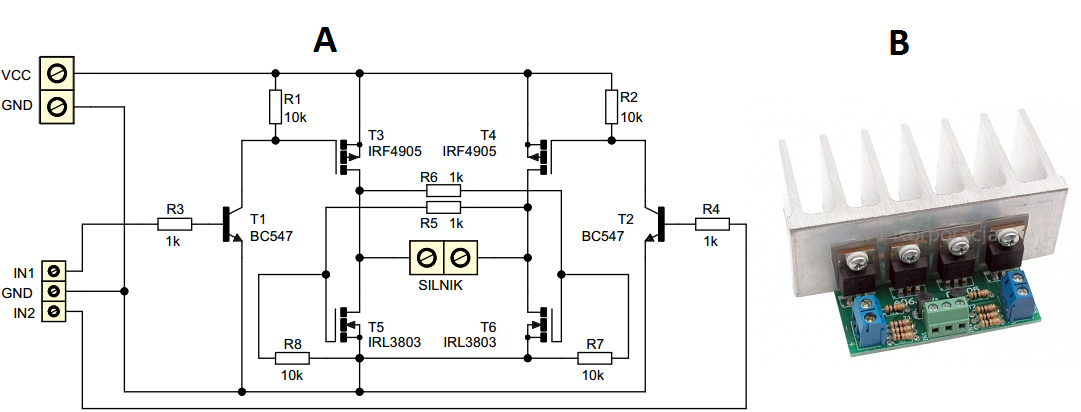
\includegraphics[scale=0.45]{imgs/mostek_h_schemat.png}
 	\caption[Schemat mostka H.]{\small{Ilustracja A przedstawia schemat ideowy mostka H, B - zdjęcie wykonanego mostka.}\footnotemark}
	\label{mostek_h_sch}
    \end{center}
  \end{figure}  
  	  \footnotetext{\emph{Mostek H}, http://sklep.avt.pl/,  (data dostępu 29.12.2015 r.)}
  	  
Część logiczna zasilana jest z 5 V źródła napięcia. Na oficjalnej stronie \textit{Raspberry Pi} napisane jest, że powinno się zastosować zasilacz o mocy około 10 W. Na pokładzie robota znajduje się 12 V bateria. Wystarczy zatem wykorzystać przetwornicę obniżającą napięcie - \textit{step-down}, która przedstawiona została na rysunku \ref{p_dc_dc_sch}. Ilustracja \ref{p_dc_dc_sch}A przedstawia schemat ideowy przetwornicy, której działanie opiera się o kluczowanie stałego napięcia wejściowego U$_1$ przy pomocy tranzystora K. Cewka L oraz kondensator C$_0$ magazynują energię dostarczoną podczas zwarcia klucza K, którą oddają w fazie rozwarcia. Zadaniem diody D jest zapewnienie odpowiedniego kierunku przepływu prądu. Napięcie wyjściowe U$_0$ odłożone na obciążeniu R$_0$ jest zależne od współczynnika wypełnienia kluczowanego napięcia. Na rysunku \ref{p_dc_dc_sch}B przedstawiona została wykorzystana przetwornica. 
\begin{figure}[H]
    \begin{center}
      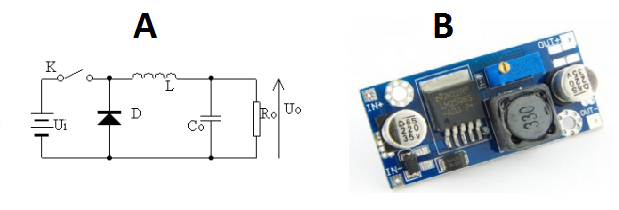
\includegraphics[scale=0.82]{imgs/przetwornica.png}
 	\caption[Przetwornica obniżająca napięcie DC/DC]{\small{Ilustracja A przedstawia schemat ideowy przetwornicy typu \textit{step-down}}\footnotemark \small{, B - zdjęcie wykorzystanej przetwornicy.}\footnotemark}
	\label{p_dc_dc_sch}
    \end{center}
  \end{figure}  
  	\footnotetext[2]{\emph{PRZETWORNICE IMPULSOWE – DŁAWIKOWE }, http://http://ue.pwr.wroc.pl/,  (data dostępu 29.12.2015 r.)}
  	  \footnotetext{\emph{Przetwornica napięcia DC-DC LM2596S}, http://http://electropark.pl/,  (data dostępu 29.12.2015 r.)}

Płytka realizująca funkcję sterownika silników napędowych została zaprojektowana od podstaw, w związku z tym posiada własny układ zasilający oparty o stabilizator liniowy 7805, którego schemat przedstawiony został na rysunku \ref{zas_at}. Zastosowany układ scalony odpowiedzialny jest przede wszystkim za obniżenie napięcia wejściowego do żądanej wartości. Dodatkowo posiada on także zintegrowane systemy chroniące go przed zwarciem oraz przegrzaniem. Układy logiczne wymagają dużej stabilności napięcia zasilającego, stąd też zarówno na wejściu jak i wyjściu układu zastosowane zostały dodatkowe kondensatory. Elementy C1, C4 to kondensatory elektrolityczne charakteryzujące się dużą pojemnością mogące skompensować stosunkowe duże wahania napięcia. C2 oraz C3 to kondensatory ceramiczne, które dobrze radzą sobie z szybkozmiennymi, niewielkimi zmianami.

  \begin{figure}[H]
    \begin{center}
      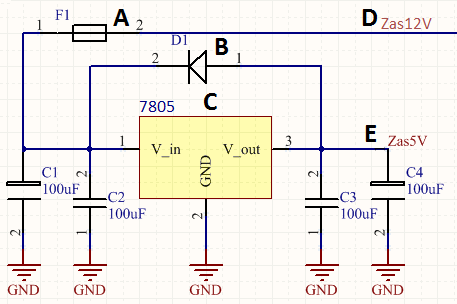
\includegraphics[scale=0.55]{imgs/zasilanie_atmeg.png}
 	\caption[Zasilanie sterownika silników.]{\small{Schemat ideowy układu zasilania, na którym: A - bezpiecznik nadmiarowo-prądowy (350mA), B - dioda mająca na celu zabezpieczenie układu przez przepięciami mogącymi pojawić się po stronie wyjściowej, C - liniowy stabilizator napięcia 7805, D - 12 V napięcie wejściowe, E - 5 V napięcie wyjściowe. Kondensatory C1, C2, C3 oraz C4 dodatkowo stabilizują napięcie.}}
	\label{zas_at}
    \end{center}
  \end{figure}  
  
Uruchomienie robota zrealizowane zostało przy wykorzystaniu pojedynczego włącznika, podłączonego szeregowo pomiędzy baterią a resztą pojazdu. Części wykonawcze robota (głównie silniki) potrafią pobierać bardzo duży prąd, w związku z tym przy wyborze elementu należy kierować się jego wytrzymałością prądową. Robot, w najgorszym przypadku, może pobierać około 13 A (silniki napędowe 2$\cdot$5 A, logika 3 A) co jest dość dużą wartością. Przełączniki mogące pracować w takich warunkach są duże i nieporęczne. Zastosowany został zatem przekaźnik wraz z układem pozwalającym na ograniczenie prądu płynącego przez jego cewkę (rys. \ref{wyla}). Robot uruchamiany jest ręcznie przy wykorzystaniu przełącznika suwakowego A. Jego załączenie powoduje przepływ prądu przez cewkę przekaźnika B. Nominalny prąd płynący cewki w zastosowanym przekaźniku wynosi 30 mA, jednakże ,,pełną moc" cewki wykorzystuje się tylko w momencie załączenia styku - czyli bezpośrednio po włączeniu zasilania. Podtrzymywanie go w tej pozycji nie wymaga już tak dużego pola magnetycznego. Zastosowanie układu złożonego z rezystancji R oraz pojemności C pozwala na zmniejszenie prądu prądu płynącego przez układ. W chwili załączenia, gdy kondensator jest nienaładowany, traktowany jest jako zwarcie - przez układ płynie pełny prąd. Po chwili, gdy pojemność C się naładuje, jest ona rozwarciem, więc prąd będzie płynąć przez rezystancję R - będzie miał mniejszą wartość. Zastosowanie obciążenia o wartości odpowiadającej rezystancji cewki, czyli 400$\Omega$, zmniejsza jego wartość o połowę.

  \begin{figure}[H]
    \begin{center}
      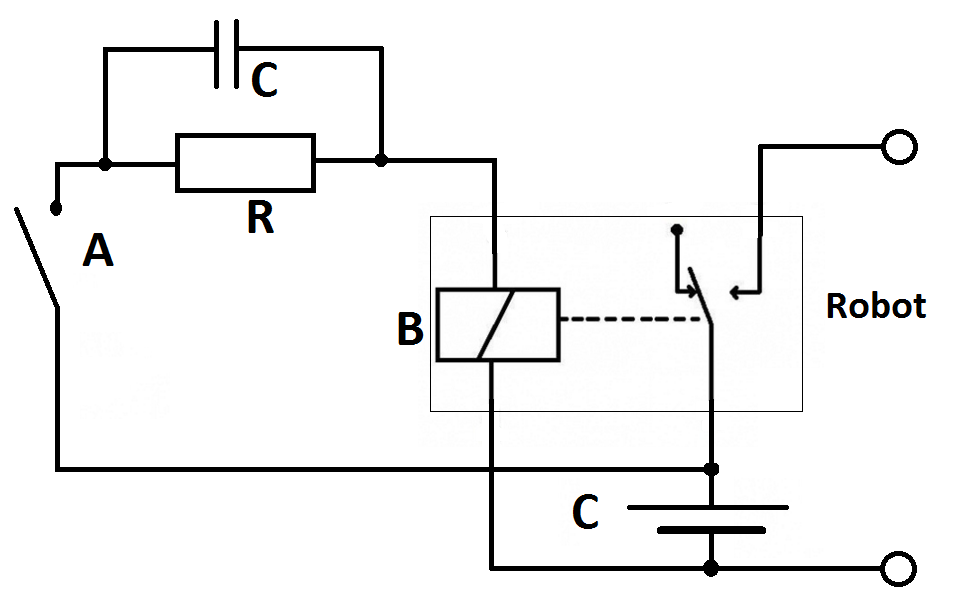
\includegraphics[scale=0.28]{imgs/wylaczniik.png}
 	\caption[Wyłącznik główny.]{\small{Schemat ideowy włącznika głównego zrealizowanego przy wykorzystaniu przekaźnika - B. Pozostałe elementy to: A - niewielki przełącznik suwakowy, C - bateria, R - rezystor, C - kondensator.}}
	\label{wyla}
    \end{center}
  \end{figure}   
  
  \namedsection{Podłączenie silników napędowych}
  Silniki sterowane są przez mostek H, który jest zbudowany w oparciu o tranzystory polowe. Elementy te są jednak stosunkowo wrażliwe na różnego rodzaju przepięcia oraz ładunki elektrostatyczne. Szczotkowe silniki prądu stałego w ogólności mogą być wykorzystane jako prądnice, co można zaobserwować mierząc napięcie na zaciskach obracającego się silnika. Zjawisko to może powstać w momencie odcięcia sygnału sterującego mostkiem H. Bezwładność pojazdu jeszcze przez chwilę będzie powodować obracanie się kół i generowanie ładunku. Aby zniwelować wpływ tego zjawiska na tranzystory zastosowano układ pokazany na rysunku \ref{diody}. Do tego celu wykorzystane zostały diody Schottky'ego, charakteryzujące się przede wszystkim niższym napięciem polaryzacji złącza p-n wynoszącym około 0,4~V.

  \begin{figure}[H]
    \begin{center}
      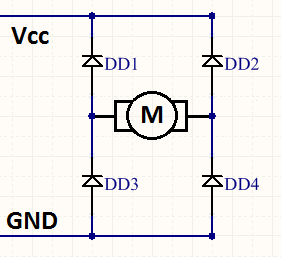
\includegraphics[scale=0.7]{imgs/silnik_pol.png}
 	\caption[Podłączenie silników napędowych.]{\small{Schemat ideowy układu odprowadzającego nadmiarowy ładunek z obwodu silników napędowych. Przedstawione elementy: DD1, DD2, DD3 oraz DD4 - diody Schottky'ego, Vcc - napięcie z baterii, GND - masa układu.}}
	\label{diody}
    \end{center}
  \end{figure}   
  
  \namedsection{Eliminacja drgań styków}
  Na płytce drukowanej znajdują się mikro przyciski oraz krańcówki, które są urządzeniami mechanicznymi - mogą wywoływać drgania podczas zwierania bądź rozwierania styków. Powstałe w ten sposób zakłócenie może niekiedy negatywnie wpływać na działanie zarówno układu jak i programu wyzwalając pewną funkcję dużą liczbę razy. Aby przeciwdziałać temu zjawisku zastosowany został sprzętowy układ eliminujący drgania, który został przedstawiony na schemacie \ref{drg}. Zaprezentowane rozwiązanie utrzymuje wysoki stan logiczny dla rozwartego, nie wciśniętego przycisku. Najważniejszym elementem układu jest kondensator, który jako element całkujący usuwa składowe wysokoczęstotliwościowe - drgania. 
  \newpage
 \begin{figure}[H]
    \begin{center}
      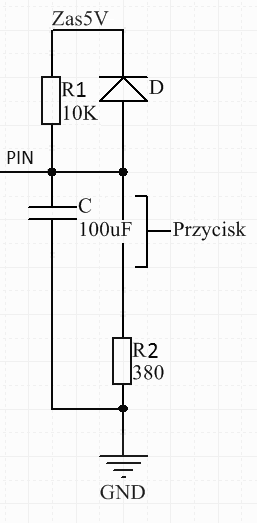
\includegraphics[scale=0.45]{imgs/drgania.png}
 	\caption[Eliminacja drgań styków.]{\small{Schemat ideowy układu eliminacji drgań styków. Rezystor R1 jest rezystorem podciągającym o wartości 10 k$\Omega$, D - dioda chroniąca układa przed przepieciami, C - kondensator, który tłumi drgania o pojemności 100 $\mu$F, R2 - rezystor ograniczający prąd zwarciowy płynący z kondensatora C po naciśnięciu przycisku o wartości 380 $\Omega$. PIN to wyprowadzenie prowadzące do wejścia mikrokontrolera. }}
	\label{drg}
    \end{center}
  \end{figure}   
  
  \namedsection{Realizacja magistrali TWI} 
  Magistrala TWI w ogólności wymaga jedynie podłączenia rezystorów podciągających dla linii komunikacyjnych co zostało przedstawione na schemacie \ref{podlaczenie_TWI}. W projekcie zastosowano do tego rezystory o wartości 4,7 k$\Omega$. Problem pojawił się jednak w przypadku wspólnego połączenia zastosowanych Atmeg48 oraz \textit{Raspberry Pi}. Mikrokontrolery pracują na napięciu 5 V - tak samo jak magistrala TWI. Druga platforma natomiast pracuje na napięciu 3,3 V. W związku z tym należało zastosować układ konwersji stanów logicznych, którego schemat został przedstawiony na schemacie \ref{konw_sch}. Minimalne napięcie umożliwiające prawidłową pracę, zgodnie z dokumentacją techniczną, wynosi $0,7\cdot 5V = 3,5 V$. Dla tego typu układów należy zastosować tranzystory (TR1 oraz TR2) dedykowane do konwersji stanów logicznych transmisji danych, czyli przystosowane do pracy przy wysokich częstotliwościach. Elementy tego typu charakteryzują się szczególnie małymi wartościami pojemności pasożytniczych.
  
\begin{figure}[H]
    \begin{center}
      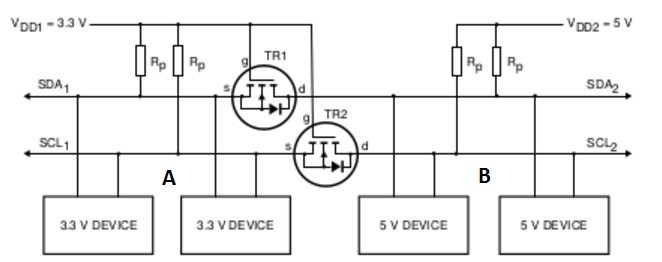
\includegraphics[scale=0.40]{imgs/konwersja.jpg}
 	\caption[Konwersja stanów logicznych.]{\small{Na rysunku przedstawiono schemat ideowy układu konwersji stanów logicznych opartego o dwa tranzystory polowe TR1 oraz TR2. Sekcja A to urządzenia pracujące z napięciem 3,3 V. Sekcja B - 5 V. Rezystory R$_p$ pełnią funkcję rezystorów podciągających.}\footnotemark}
	\label{konw_sch}
    \end{center}
  \end{figure}  
  	  \footnotetext{\emph{Raspberry Pi and I2C devices of different voltage}, http://nathan.chantrell.net/,  (data dostępu 30.12.2015 r.)}
  	  
  \namedsection{Rezonator kwarcowy}
  Rezonatory kwarcowe są układami służącymi do stabilizacji częstotliwości. Wykonane jako osobne komponenty (aby zapobiegać zakłóceniom) charakteryzują się wysoką jakością generowanego przebiegu. Ich głównym elementem jest kryształ kwarcu, który w wyniku pobudzenia polem elektrycznym zaczyna wibrować. Każdy rezonator ma ściśle określoną częstotliwość pracy, dla której występuje zjawisko rezonansu mechanicznego.  Atmega48 posiada wewnętrzny oscylator, jednakże umożliwia ona taktowanie jedynie z prędkością 8 MHz. Aby wykorzystać pełną moc układu należy zastosować rezonator kwarcowy o częstotliwości 20 MHz. Schemat przedstawiający sposób podłączenia elementu przedstawiona na rysunku \ref{xxtal}. Kondensatory C5 oraz C6 dodatkowo stabilizują ,,punkt pracy" układu. 
  
   \begin{figure}[H]
    \begin{center}
      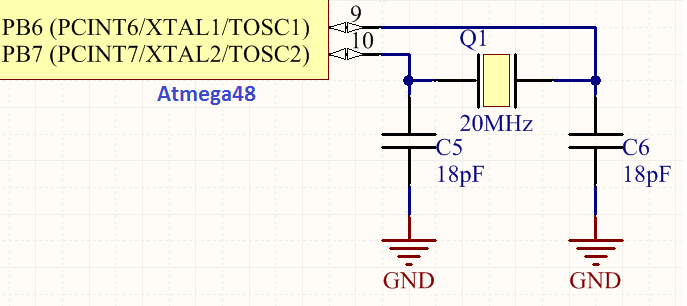
\includegraphics[scale=0.45]{imgs/xtal.png}
 	\caption[Podłączenie rezonatora kwarcowego.]{\small{Schemat ideowy przedstawia sposób podłączenia zewnętrznego oscylatora Q1 do mikrokontrolera. Wartość kondensatorów C5 oraz C6 określa dokumentacja techniczna układu. Ich zadaniem jest stabilizacja rezonansu kryształu kwarcowego. }}
	\label{xxtal}
    \end{center}
  \end{figure}   
  